\chapter{Features and Functionality}

\section{User Interface and User Experience (UI/UX) Design}

The User Interface (UI) and User Experience (UX) design of our project focus on providing an intuitive and user-friendly environment. The design principles include simplicity, clarity, and responsiveness, ensuring that users can easily interact with the simulation tool and obtain meaningful results.

Key aspects of the UI/UX design include:
\begin{itemize}
    \item \textbf{Layout:} The layout is organized with clear sections for input parameters, control buttons, and the 3D visualization area.
    \item \textbf{Interactive Controls:} Users can start, stop, pause, and reset simulations using clearly labeled buttons.
    \item \textbf{Real-time Feedback:} The UI provides real-time feedback on the status of the simulation and the state of the objects.
    \item \textbf{Customization:} Users can adjust various parameters and settings to customize the simulation to their needs.
\end{itemize}

\begin{figure}[h!]
    \centering
    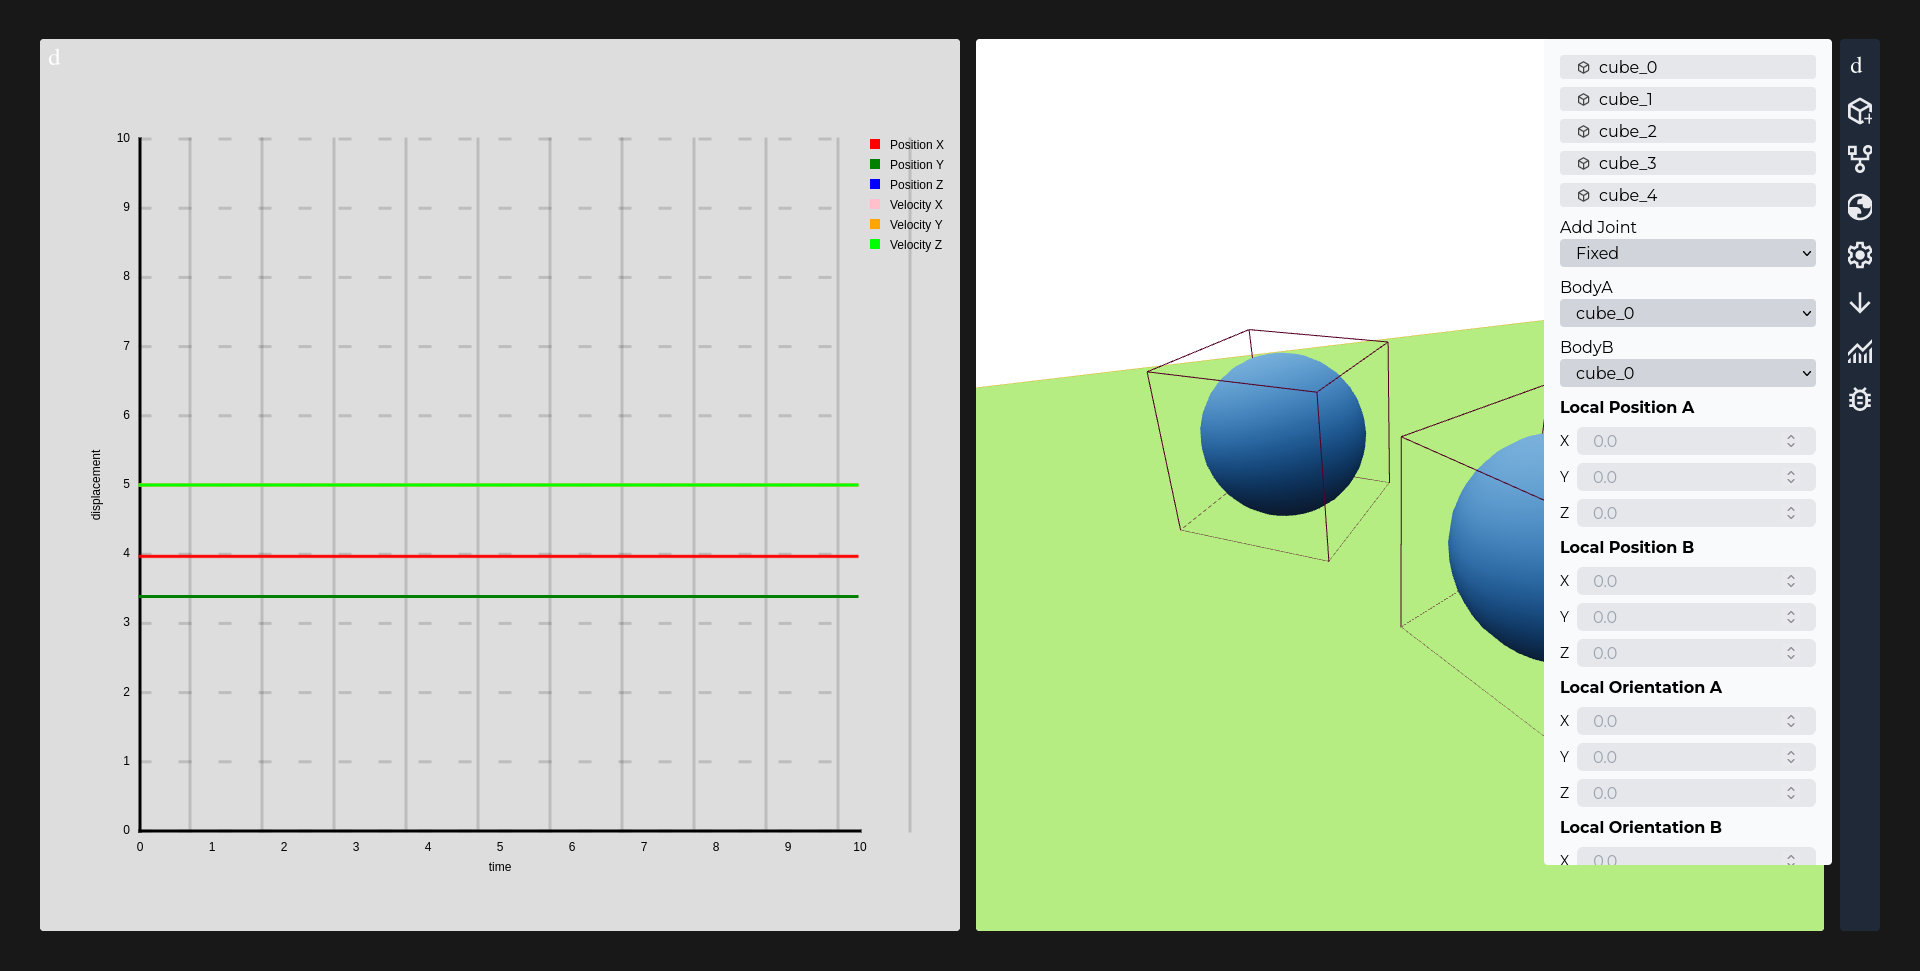
\includegraphics[width=\textwidth]{ui_design.png}
    \caption{User Interface Design}
    \label{fig:ui_design}
\end{figure}

\section{Core Features of the App}

The core features of the app include:
\begin{itemize}
    \item \textbf{Real-time Simulation:} Perform real-time simulations of physical systems with accurate physics calculations.
    \item \textbf{3D Visualization:} Visualize simulations in a three-dimensional space, providing a realistic view of the modeled systems.
    \item \textbf{Interactive Controls:} Control the simulation with start, stop, pause, and reset functionalities.
    \item \textbf{Customizable Parameters:} Adjust parameters such as mass, force, friction, and other properties to explore different scenarios.
    \item \textbf{Predefined Scenarios:} Load and simulate predefined scenarios, such as the quarter car model, pendulum, and mass spring system.
\end{itemize}

\section{Description of Different Modules and Their Functionalities}

The app is divided into several modules, each responsible for specific functionalities:

\subsection{User Interface (UI) Module}

The UI module provides the front-end interface for users to interact with the app. It includes input fields for parameters, control buttons, and the 3D visualization area.

\subsection{Physics Engine Module}

The Physics Engine module handles the core physics calculations. It computes forces, updates object states, and handles collisions. This module ensures that the simulations are accurate and realistic.

\subsection{3D Rendering Module}

The 3D Rendering module is responsible for visualizing the simulation results. It renders objects in a three-dimensional space using Three.js, handling lighting, shading, and camera controls.

\subsection{Scenario Manager Module}

The Scenario Manager module allows users to load and save predefined scenarios. It manages the setup of different simulations, including the quarter car model, pendulum, and mass spring system.

\section{Example Scenarios and Simulations}

The app includes several predefined scenarios to demonstrate its capabilities:

\subsection{Simple Pendulum}
The pendulum scenario simulates the motion of a simple pendulum. It includes a mass attached to a string or rod, swinging under the influence of gravity.

\begin{figure}[h!]
    \centering
    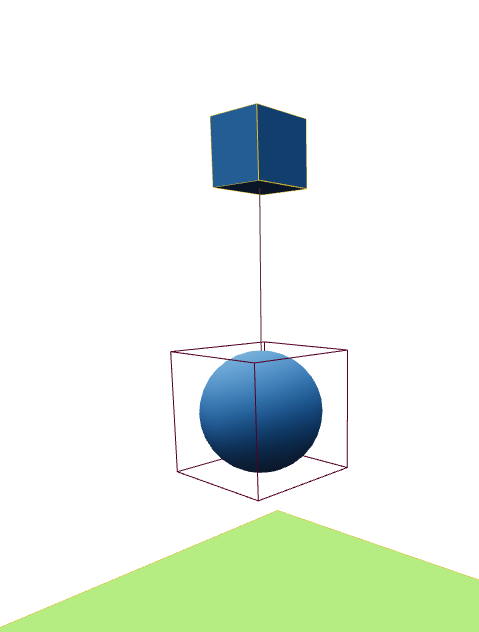
\includegraphics[width=0.3\textwidth]{pendulum.png}
    \caption{Pendulum Simulation}
    \label{fig:pendulum}
\end{figure}



